%%%%%%%%%%%%%%%%%%%%%%%%%%%%%%%%%%%%%%%%%%%%%%%%%%%%%%%%%%%%%%%%%%%%%%%%%%%%%%%%%%%%%%%%%
% Projekt: AIiR																		%
% Semestr VI																			%
% Data: Marzec / Czerwiec 2015															%
%%%%%%%%%%%%%%%%%%%%%%%%%%%%%%%%%%%%%%%%%%%%%%%%%%%%%%%%%%%%%%%%%%%%%%%%%%%%%%%%%%%%%%%%%

%----------------------------------------------------------------------------------------
% PREAMBUŁA: PAKIETY I KONFIGURACJA DOKUMENTU
%----------------------------------------------------------------------------------------

\documentclass[a4paper,12pt]{article}		% klasa dokumentu i rozmiar czcionki
\usepackage[utf8]{inputenc}					% kodowanie uniwersalne
\usepackage[margin=2.5cm]{geometry}			% określa wielkość marginesów
\usepackage{polski}							% polski pakiet językowy
\usepackage{fancyhdr}						% nagłówek i stopka
\usepackage{lastpage}						% potrzebny fancyhdr do numerowania
\usepackage{extramarks}						% potrzebny fancyhdr
\usepackage{amsmath}						% wzory matematyczne
\usepackage{relsize}						% zmiana wielkości wzorów matematycznych
\usepackage{booktabs}						% do tabel
\usepackage{multirow}						% do łączenia wierszy w tabeli
\usepackage{multicol}						% do łączenia kolumn w tabeli
\usepackage{placeins}						% do stawiania "barier" tabeli
\usepackage{graphicx}						% załączanie obrazów
\usepackage{caption}						% zarządzanie podpisami pod floatami
\usepackage{gensymb}						% znaki specjalne
\usepackage[parfill]{parskip}				% dodaje pustą linię między paragrafami
\usepackage{hyperref}						% links
\usepackage{url}							% generowanie linków ze znakami specjalnymi
\usepackage{pdflscape}						% zmiana orientacji strony
\usepackage{indentfirst}					% dodanie pierwszego wcięcia w tekście
\usepackage{listings}
\usepackage{color}
 
\definecolor{codegreen}{rgb}{0,0.6,0}
\definecolor{codegray}{rgb}{0.5,0.5,0.5}
\definecolor{codepurple}{rgb}{0.58,0,0.82}
\definecolor{backcolour}{rgb}{0.95,0.95,0.92}
 
\lstdefinestyle{mystyle}{
    backgroundcolor=\color{backcolour},   
    commentstyle=\color{codegreen},
    keywordstyle=\color{magenta},
    numberstyle=\tiny\color{codegray},
    stringstyle=\color{codepurple},
    basicstyle=\footnotesize,
    breakatwhitespace=false,         
    breaklines=true,                 
    captionpos=b,                    
    keepspaces=true,                 
    numbers=left,                    
    numbersep=5pt,                  
    showspaces=false,                
    showstringspaces=false,
    showtabs=false,                  
    tabsize=2
}
 
 \lstset{style=mystyle}
%----------------------------------------------------------------------------------------
% PREAMBUŁA: DEFINICJE KOMED DLA NAGŁÓWKA I STOPKI
%----------------------------------------------------------------------------------------

\newcommand{\AuthorName}{Sternik,Cichuta,Cebula,Sygut}
\newcommand{\Title}{Obliczanie przybliżenia liczby Pi.}
\newcommand{\UnderTitle}{Dokumentacja końcowa}
\newcommand{\University}{Politechnika Wrocławska}
\newcommand{\Class}{Aplikacje Internetowe i Rozproszone}
\newcommand{\ClassDay}{Środa}
\newcommand{\ClassTime}{07:30}
\newcommand{\ClassInstructor}{dr inż.~Marek Woda}

%----------------------------------------------------------------------------------------
% PREAMBUŁA: DEFINICJE KOMEND
%----------------------------------------------------------------------------------------

\renewcommand{\baselinestretch}{1.20}				% wielkość odstępu między wierszami
\renewcommand\headrulewidth{0.4pt}					% wielkość nagłówka
\renewcommand\footrulewidth{0.4pt}					% wielkość stopki
\newcommand{\HRule}{\rule{\linewidth}{0.5mm}}		% szerokość poziomego paska

%----------------------------------------------------------------------------------------
% PREAMBUŁA: USTAWIENIA NAGŁÓWKA I STOPKI
%----------------------------------------------------------------------------------------

\pagestyle{fancy}										% styl strony stosujący fancyhdr
\lhead{Obliczanie liczby Pi}							% górny-lewy
\rhead{\Class}											% górny-prawy
\rfoot{Strona\ \thepage\ z\ \protect\pageref{LastPage}}	% dolny-prawy

%----------------------------------------------------------------------------------------
% PREAMBUŁA: INNE USTAWIENIA
%----------------------------------------------------------------------------------------

\setlength{\parindent}{1cm} 							% szerokość wcięć w paragrafach

%----------------------------------------------------------------------------------------
% PDF META INFO
%----------------------------------------------------------------------------------------

\pdfinfo
{
	/Author (\AuthorName)
	/Title (\Class \Title)
	/CreationDate (\today)
	/Subject (\Class)
	/Keywords (\Class, \Title, LaTeX)
}

%----------------------------------------------------------------------------------------
% STRONA TYTUŁOWA: SEKCJA NAGŁÓWKA
%----------------------------------------------------------------------------------------

\begin{document}
\begin{titlepage}
\hfill Wrocław, dn. 10 czerwca 2015r.\\
\center
\textsc{}\\[1.5cm]
\textsc{\LARGE \University}\\[1.5cm]
\textsc{\Large \Class}\\[1.5cm]

%----------------------------------------------------------------------------------------
% STRONA TYTUŁOWA: SEKCJA TYTUŁU
%----------------------------------------------------------------------------------------

\HRule \\[0.7cm]
{ \huge \bfseries \Title}\\[0.4cm]
\textsc{\large \UnderTitle}\\[0.5cm]
\HRule \\[1.0cm]

%----------------------------------------------------------------------------------------
% STRONA TYTUŁOWA: SEKCJA AUTORA
%----------------------------------------------------------------------------------------

\begin{minipage}{0.5\textwidth}
\begin{flushleft} \large
\emph{Grupa projektowa:}
\\ Paweł \textsc{Sternik}, 200623
\\ Kamil \textsc{Cichuta}, ???
\\ Mariusz \textsc{Cebula}, ???
\\ Sławomir \textsc{Sygut}, ???
\end{flushleft}
\end{minipage}
~
\begin{minipage}{0.4\textwidth}
\begin{flushright} \large
\emph{Prowadzący:}
\\ dr inż.~Marek \textsc{Woda}
\end{flushright}
\end{minipage}\\[3cm]

%----------------------------------------------------------------------------------------
% STRONA TYTUŁOWA: SEKCJA DATY
%----------------------------------------------------------------------------------------

\emph{Termin spotkań:}\\[0.35cm]
{\large \ClassDay, godz. \ClassTime}\\[0.5cm]
\vfill
\end{titlepage}

%----------------------------------------------------------------------------------------
% SPIS TREŚCI
%----------------------------------------------------------------------------------------

\newpage
\tableofcontents
\newpage

%----------------------------------------------------------------------------------------
% DOKUMENT: SEKCJA
%----------------------------------------------------------------------------------------

\section{Temat projektu.}
Tematem projektu realizowanego w ramach kursu Aplikacje Internetowe i Rozproszone było wyznaczanie rozszerzenia liczby Pi z wykorzystaniem algorytmu Monte Carlo. Realizacja wymagała implementacji kilku modułów stanowiących cały system.
\section{Cel projektu.}
\subsection{Cel dydaktyczny.}
Głównym celem dydaktycznym kursu było zapoznanie się z technologiami wykorzystywanymi do tworzenia rozproszonych aplikacji połączonych z internetowymi klientami. Ponadto kurs wymagał zoorganizowania pracy w grupach kilkuosobowych co wymuszało zaplanowanie kolejnych etapów pracy i podział poszczególnych zadań między członków grupy. Wykorzystane zostały do tego odpowiednie narzędzia komunikacji, które zostaną opisane dokładniej w dalszej częsci dokumentu. 
\subsection{Cel merytoryczny.}
Implementacja algorytmu Monte Carlo obliczającego rozszerzenie liczby Pi z wykorzystaniem technologi MPI (ang. Message Passing Interface ) czyli protokołu komunikacyjnego służącego do przesyłania komunikatów pomiędzy procesami programów równoległych. Ponadtwo stworzenie aplikacji internetowej która poprzez stworzoną bazę dancyh łączy się z silnikiem obliczeniowym działającym na kilku niezależnych komputerach. Strona powinna posiadać elementy zmieniające się dynamicznie podczas realizacji zadania - przykładowo pasek postępu. 
\newpage
\section{Opis zastosowanego algorytmu.}
\subsection{Opis słowny algorytmu.}
Metoda Monte Carlo stosowana jest do problemów, które jest bardzo trudno rozwiązać za pomocą podejścia analitycznego. Najczęściej stosuje się ją do modelowania złożonych problemów takich jak: 
\begin{enumerate}
\item Obliczanie całek.
\item Obliczanie łańcuchów procesów statystycznych .
\item Obliczanie złożonych symulacji.
\end{enumerate}
Metoda opiera się na losowaniu nazywanym w tym przypadku wyborem przypadkowym. Losowanie dokonywane jest zgodnie z rozkładem, który jest znany. Przykładowo całkowanie metodą Monte-Carlo działa na zasadzie porównywania losowych próbek z wartością funkcji. Dokładność wyniku uzyskanego tą metodą jest zależna od liczby sprawdzeń i jakości użytego generatora liczb pseudolosowych. Zwiększanie liczby prób nie zawsze zwiększa dokładność wyniku, ponieważ generator liczb pseudolosowych ma skończenie wiele liczb losowych w cyklu. Przykładowo całkowanie tą metodą jest używane w przypadkach, kiedy szybkość otrzymania wyniku jest ważniejsza od jego dokładności (np. obliczenia inżynierskie).\\

W projekcie algorytm Monte Carlo zostanie wykorzystany do obliczenia rozszerzenia dziesiętnego liczby Pi. Dokładny opis realizacji tego algorytmu znajduję się w następnym punkcie.
\subsection{Obliczanie liczby Pi metodą Monte Carlo.} 
Liczbę Pi można obliczać na wiele różnych sposobów. Jednym z nich jest wykorzystanie metody Monte Carlo. Metoda ta charakteryzuję się przede wszystkim swoją stosunkową prostą procedurą jak i przystosowaniem do zaimplementowania mechanizmów zrównoleglenia - co jest jednym z głównych celów projektu.
\begin{figure}[h!]
\centering
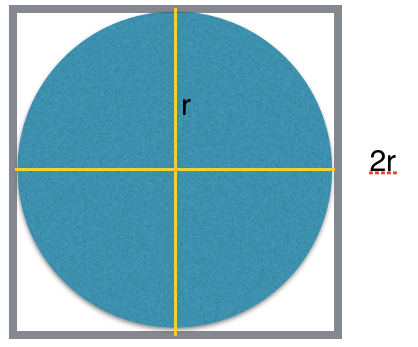
\includegraphics[scale=0.5]{Resources/Kolo_rysunek.png}
\caption{Koło o promieniu r wpisane w kwadrat - bok 2r.}
\end{figure}
Pole kwadratu przedstawionego na Rysunku 1 wynosi:
 \[(4\prod)^{2}\]
 natomiast koła oczywiście:
 \[(\prod)r^{2}\]
 \newpage
 Znając zatem pole koła jak i kwadratu można zauważyć że stosunek pola koła do pola kwadratu wynosi:
\[ \frac{PoleKola}{PoleKwadratu}=\frac{\prod r^{2}}{4r^{2} }= \frac{\prod}{4}\]
Następnie korzystając z tego, że pole koła jak i kwadratu zostały w jakiś sposób obliczone można wyciągnąć wzór na liczbę Pi:
\[\prod =4\frac{PoleKola}{PoleKwadratu}\]
Dojście do tego punktu mogłoby się wydawać zatoczeniem koła i powrotem do punktu początkowego problemu. Tak nie jest. Ponieważ dopiero w tym miejscu pojawia się cała charakterystyka metody Monte Carlo. Abstrakcyjnie należy sobię teraz wyobraźić sytuację, w której rzucamy bardzo dużo razy rzutkami w tarczę wyglądająca jak Rysunek 1. Kończąc grę, plansza będzie pokryta rzutkami znajdującymi sie we wnętrzu koła jak i poza nim na obszarze kwadratu. Podsumowując liczba rzutek w i poza kołem będzie równa stosunkowi pola koła do pola kwadratu.
\begin{figure}[h!]
\centering

\includegraphics[scale=0.7]{Resources/Losowanie.png}
\caption{Przykład losowania punktów.}
\end{figure}
 Formalnie losowanie będzie odbywać się pośród punktów należących do zbioru pokrytego współrzędnymi należacymi do predziału [-2r,2r]. Stosunek liczby punktów
zawierających się w kole o środku w punkcie [0,0] i promieniu r do wszystkich wylosowanych punktów będzie dążył w nieskończoności (z pewnym prawdopodobieństwem) do stosunku tego pola koła do koła kwadratu o boku 2r. Co więcej, stosunek ten będzie identyczny również do ćwiartki koła. Jeżeli pole koła podzielimy na cztery i tak samo podzielimy pole kwadratu, to ich stosunek będzie wciąż taki sam. Oznacza to, że wystarczy, jeżeli będziemy losowali punkty o współrzędnych od 0 do r. Cała metoda sprowadza się więc do tego, by losować punkty, sprawdzać, czy mieszczą się w kole, i następnie podstawiać liczby wylosowanych punktów do wzoru. Losując odpowiednio dużo punktów, powinniśmy otrzymać z pewnym prawdopodobieństwem rozsądne przybliżenie liczby Pi.
\subsection{Implementacja algorytmu - program jednowątkowy.} 
Dla lepszego zrozumienia działania algorytmu i sprawdzenia jego rezultatów stworzony został program w języku C++ obliczający przybliżenie liczby Pi wykonujący wszystkie obliczenia szeregowo, czyli po prostu korzystający z jednego wątku. Program przyjmuje od użytkownika zadaną liczbę punktów. W rezultacie wyświetla obliczoną liczbę Pi oraz orginalne rozwinięcie.
\lstinputlisting[language=C++]{Code/obliczanie_pi.cpp}
\begin{figure}[h!]
\centering
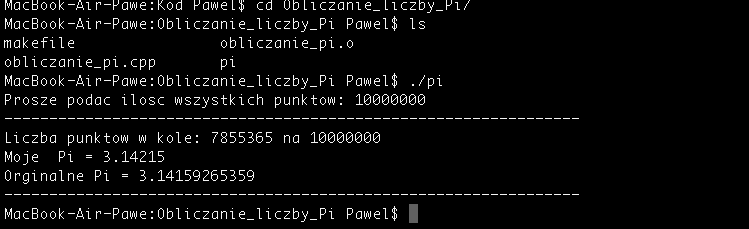
\includegraphics[scale=0.6]{Resources/Screen_Program_JedenWatek}
\caption{Przykład działania programu jednowątkowego.} 
\end{figure}
Jak widać na zamieszczonym zdjęciu ekranu program jednowątkowy obliczający rozwinięcie dziesiętne liczby Pi korzystając z metody Monte Carlo obliczył liczbę Pi równą 3.14215. Otrzymana dokładność sięga jedynie dwóch miejsc po przecinku przy stosunkowo już dużej ilości losowanych punktów - 10 mln. Program wyświetlił informację o tym, że 7855365 punktów znalazło się w kole.
\section{Zastosowane technologie.}
\subsection{Framework Django.}
\subsubsection{Opis.}
Django – wysokopoziomowy, opensource’owy framework przeznaczony do tworzenia aplikacji internetowych, napisany w Pythonie. Powstał pod koniec 2003 roku jako ewolucyjne rozwinięcie aplikacji internetowych, tworzonych przez grupę programistów związanych z Lawrence Journal-World. Nazwa frameworku pochodzi od imienia gitarzysty Django Reinhardta.
Framework wymaga instalacji interpretera Pythona. W ramach projektu wykorzystany został Python 2.7.6, instalacja jednak nie była konieczna, ponieważ w systemie Linux był wgrany domyślnie.
\subsubsection{Instalacja Django.}
W projekcie zostało użyte Django w wersji 1.7.5, jednak od 01.04.2015 dostępna jest już wersja 1.8 LTS:\\
\textbf{pip install Django==1.7.5}
\subsubsection{Tworzenie nowego projektu.}
W linii poleceń należy przejść do katalogu, w którym będzie znajdował się kod, następnie wpisując:\\
\textbf{django-admin.py startproject PI}\\
Utworzony zostanie katalog z projektem:
PI/\\
init.py\\
manage.py\\
settings.py\\
urls.py
\begin{itemize}
\item \textbf{init.py: }Pusty plik informujący Pythona o tym, że katalog nadrzędny powinien być traktowany jako pakiet Pythona 
\item \textbf{manage.py: }Działające z linii poleceń narzędzie, które pozwala na interakcję z projektem Django na różne sposoby.
\item \textbf{settings.py}Ustawienia/konfiguracja dla tego projektu Django.
\item \textbf{urls.py}Deklaracja adresów URL dla tego projektu Django; “mapa serwisu” Twojej strony zbudowanej w oparciu o Django.
\end{itemize}
Przechodząc do katalogu PI, można sprawdzić czy server deweloperski działa, w tym celu należy wpisać:\\
\textbf{python manage.py runserver}
\subsubsection{Ustawienia bazy danych.}
Django można używać bez bazy danych, jednak dostarczony jest wraz z systemem ORM (odwzorowanie relacyjno-obiektowe), za pomocą, którego można definiować tabele w bazie danych oraz pracować na nich pisząc i operując na klasach w Pythonie. Django współpracuje z następującymi serwerami bazodanowymi: PostgreSQL, MySQL, Oracle i SQLite. Ze względu na łatwość obsługi wybrany został MySQL, przez co należało doinstalować MySQLdb:\\
\textbf{sudo apt-get install python2.7-mysqldb}\\
Co wymagało również zmiany silnika bazy danych w ustawieniach aplikacji na „django.db.backends.mysql” oraz z wnętrza powłoki bazy danych utworzenia 
potrzebnej bazy danych. Ze względu, że w pliku settings.py INSTALLEDAPPS zawarte są domyślne aplikacje, należy użyć komendy:\\
\textbf{python manage.py syncdb, która dla w/w aplikacji tworzy tabele w bazie.}
\subsubsection{Tworzenie modeli.}
W katalogu PI, aby zacząć pracę nad projektem należy wprowadzić następujące polecenie:\\
\textbf{python manage.py startapp PI2}\\
Co utworzy podkatalog PI2, w którym będzie się znajdować struktura docelowej aplikacji.
\subsection{Technologia MPI.}
MPI, czyli Message Passing Interface jest protokołem komunikacyjnym będącym standardem przesyłania komunikatów pomiędzy procesami programów równoległych działających na jednym, lub wielu komputerach. Ze względu na dominacje wykorzystywania tego modelu w klastrach komputerowych oraz superkomputerach, posłużył on jako główny protokół komunikacyjny w projekcie.
MPI jest specyfikacją biblioteki funkcji opartych na modelu wymiany komunikatów dla potrzeb programowania równoległego. Transfer danych pomiędzy poszczególnymi procesami programu wykonywanymi na procesorach maszyn będących węzłami klastra odbywa się za pośrednictwem sieci. Opisany schemat działania ilustruje poniższy rysunek.

\begin{figure}[h!]
\centering
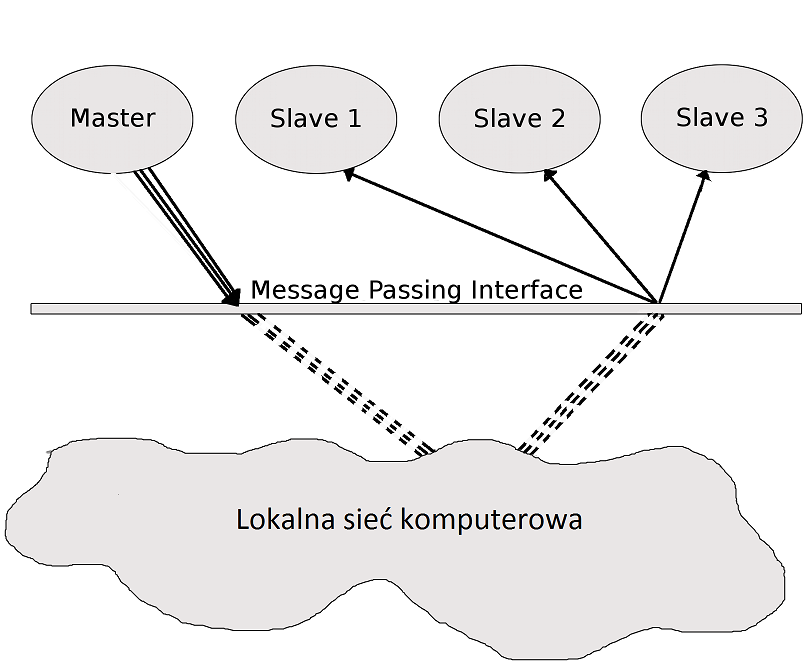
\includegraphics[scale=0.6]{Resources/mpi.jpg}
\caption{Ogólny schemat działania protokołu MPI.} 
\end{figure}

Aby zapewnić sprawną komunikacją pomiędzy komputerem Master, a Slave’ami należy skonfigurować bez kluczowe połączenia. Do tego celu najlepszym rozwiązaniem jest użycie SSH, które umożliwi logowanie bez użycia hasła, wykorzystując do tego klucz publiczny, na przykład RSA. Podstawowy schemat działania wygląda następująco:
\begin{itemize}
\item \textbf{sudo apt-get install openssh-server} - instalacja serwera ssh na komputerze Master
\item \textbf{sudo apt-get install openssh-client} - instalacja klientów na komputerach Slave
\item \textbf{ssh-keygen –t rsa} - wygenerowanie kluczy na komputerze Master
\item \textbf{scp .ssh/id\_rsa.pub username@IP\_addr:~} - skopiowanie klucza publicznego do Slave'a
\item \textbf{cat id\_rsa.pub >> .ssh/authorized\_keys} - z poziomu Slave'a dodanie otrzymanych kluczy publicznych do  kluczy autoryzowanych
\end{itemize}

Mając skonfigurowane połączenie pomiędzy hostami, można skompilować program wydając polecenie: 

\begin{itemize}
\item \textbf{mpicc pi.c –o pi.out}
\end{itemize}

Po poprawnym i bezbłędnym skompilowaniu kodu, powinien pojawić się plik wynikowy z rozszerzeniem \textbf{.out}, który należy skopiować do wszystkich hostów:

\begin{itemize}
\item \textbf{scp pi.out username@ip\_addr:~}
\end{itemize}

Jeśli wszystkie hosty posiadają ten sam program, przed uruchomieniem klastra należy stworzyć i skonfigurować plik, zawierający konfigurację maszyn w klastrze. Tworzymy plik, np. .mpi\_hostfile, który należy uzupełnić według podanego schematu:

\begin{lstlisting}
#Hostfile dla Open MPI

#Master node, parametr 'slots=2' ustawiony, dlatego, ze node jest dwu-procesorowy
localhost slots=2

#Definiujemy slave'y, oraz dozwolona liczbe procesorow do uzycia
cichy@192.168.1.118 slots=2 max_slots=4
slawek@192.168.1.119 slots=8 max_slots=8
\end{lstlisting}

Jeśli wszystko przebiegło pomyślnie możliwe jest uruchomienie programu rozproszonego:
\begin{itemize}
\item \textbf{mpirun –np liczbaProcesorow –hostfile nazwaHostfile /sciezka/pi.out}
\end{itemize}
\subsection{CSS i HTML.}
\subsection{Komunikacja grupy.}
Podczas realizacji projektu wykorzystane zostały narzędzia ułatwiające pracę w grupie. Stworzone zostało repozytorium, w którym umieszczane były kody źródłowe programu obliczającego liczbę Pi czy też apliakcji internetowej napisanej w frameworku Django. Ponadto na portalu Trello istniała tablica na której zamieszczane były zadania do zrealizowania. Umożliwiło to jasny podział zadań oraz bez problemową serializację efektów pracy niwelując liczbę konfliktów podczas równoległego tworzenia kodu przez różne osoby. Podczas realizacji projektu każdy członków z grupy dzięki dobrze zoorganizowanej tablicy Trello znał swoje zadania oraz terminy realizacji, które stanowiły motywację do pracy.
\subsubsection{GitHub.}
\begin{figure}[h!]
\centering

\includegraphics[scale=0.6]{Resources/GitHub_Logo.jpg}
\caption{Logo portalu GitHub.} 
\end{figure}
GitHub to serwis internetowy wykorzystywany masowo przy projektach programistycznych, korzystający z systemu kontroli wersji Git. Stworzony został już w 2008 roku przy wykorzystaniu języków Ruby on Rails oraz Erlang. Dzisiaj serwis obsługuje już kilka milionów repozytoriów, a wśród nich darmowe publiczne repozytoria oraz płatne prywatne. Darmowe repozytoria utrzymywane są na licencji open source. Podczas realizacji projektu został stworzony bardzo prosty tutorial korzystania z Git'a z poziomu konsoli poleceń. Tutorial opisuje korzystanie z podstawowych funkcjonalności systemu kontroli wersji , wyłączając bardziej zaawansowane techniki branch'owania i merge'owania projektów.
\begin{figure}[h!]
\centering

\includegraphics[scale=0.4]{Resources/Git_Logo.jpg}
\caption{Logo systemu kontroli wersji- Git.} 
\end{figure} 
Instrukcja do skonfigurowania i uruchomienia repozytorium opartego o system kontroli wersji Git na systemie Linux:
\begin{enumerate}
\item Instalacja najnowszej wersji gita za pomocą komendy:\\
\textbf{sudo apt-get install git}
\item Drugi krok to ustawienie globalnych danych konta założonego na stronie GitHub:\\
\textbf{sudo git config --global user.name "nazwaKonta" }
\item Następnie podajemy analogicznie maila na którego mamy zalożone konto na GitHub:\\
\textbf{sudo git config --global user.email "email"}
\item Przed tym krokiem zostały już skonfigurowane dane konta.  Teraz należy je potwierdzić i polączyć się z interesującym nas repozytorium. Do nawiązania połączenia wykorzystywane są dwa sposoby : protokół HTTPS lub SSH. Tym razem wykorzystany będzie protokół HTTPS.
\item Prawdopodobnie po skonfigurowaniu danych konta Git pobierze automatycznie repozytoria, do których dane konto miało dostęp i umieści je w folderze Dokumenty.
\item W innym przypadku należy skopiować adres repozytorium ze strony portalu. Przykładowo:\\
\textbf{https://github.com/syguts/AIiR0730obliczanieliczbyPI.git}
\item Nawiązanie połączenia poprzez komendę:\\
\textbf{git clone https://github.com/syguts/AIiR0730obliczanieliczbyPI.git AIIR}
Gdzie "AIIR" to nazwa folderu, do którego zostanie pobrane repozytorium (wersja lokalna).
\end{enumerate}
Natomiast same edytowanie repozytorium sprowadza się do sekwencji:\\
\begin{enumerate}
\item \textbf{git fetch} - funkcja sprawdza wersje zdalnego repozytorium (jeżeli zdalna wersja jest identyczna co do lokalnej wówczas wyświetlany jest stosowny komunikat)
\item \textbf{git log} - metoda wyświetla listę wprowadzonych zmian
\item \textbf{git pull} - pobranie wprowadzonych zmian - zaaktualizowanie lokalnego repozytorium.
\item \textbf{git add} -  w przypadku dodania plików należy podłączyć je pod system kontroli wersji metodą git add nazwaPlikuFolderu
\item \textbf{git status} - metoda listująca zmiany wprowadzone przez użytkownika w wersji lokalnej od ostatniej aktualizacji
\item \textbf{git commit} - stworzenie commita zbierającego wprowadzone zmiany
\item \textbf{git push} - wypchanie wprowadzonych zmian na zewnątrz lokalnego repo, czyli dodanie do zdalnego repozytorium.  
\end{enumerate}
\subsubsection{Trello.}
\begin{figure}[h!]
\centering

\includegraphics[scale=0.6]{Resources/Trello_Logo.png}
\caption{Logo portalu Trello.} 
\end{figure} 
Trello to aplikacja do zarządzania zadaniami. Opiera się ona na paradygmacie Kanban stworzonym w Japoni, w firmie Toyota, należącym do technik Agile. Trello to także produkt horyzontalny. Co to znaczy?. Oznacza to, że nie jest to produkt skierowany konkretnie do jednej grupy odbiorców, a wszystkich, którzy potrzebują danego narzędzia oraz chcących skorzystać z jego funkcji. Projekty w Trello zbudowane są w oparciu o tablice, na których to znajdują się listy zadań. Listy te pozwalają tworzyć karty (zadania), które w bardzo prosty sposób możemy sortować, czy przenosić pomiędzy różnymi listami za pomocą techniki drag-and-drop. Poszczególni użytkownicy mogą być przypisywani do kart oraz budować grupy, a grupy i konkretne projekty tworzą organizacje.Bardzo przydatną funkcjonalnością Trello są także powiadomienia, które spływają w formie wiadomości na adres email lub powiadomień (push) na urządzenia mobilne. Każdy użytkownik ma oczywiście kontrolę nad nimi oraz ich częstotliwością. Dzięki powiadomieniom można być informowanym o dyskusjach, w których pojawia się nazwa użytkownika, obserwowanych projektach, lub aktywnościach innych użytkowników. W ten sposób komunikacja następuje w błyskawicznym tempie.
\begin{figure}[h!]
\centering
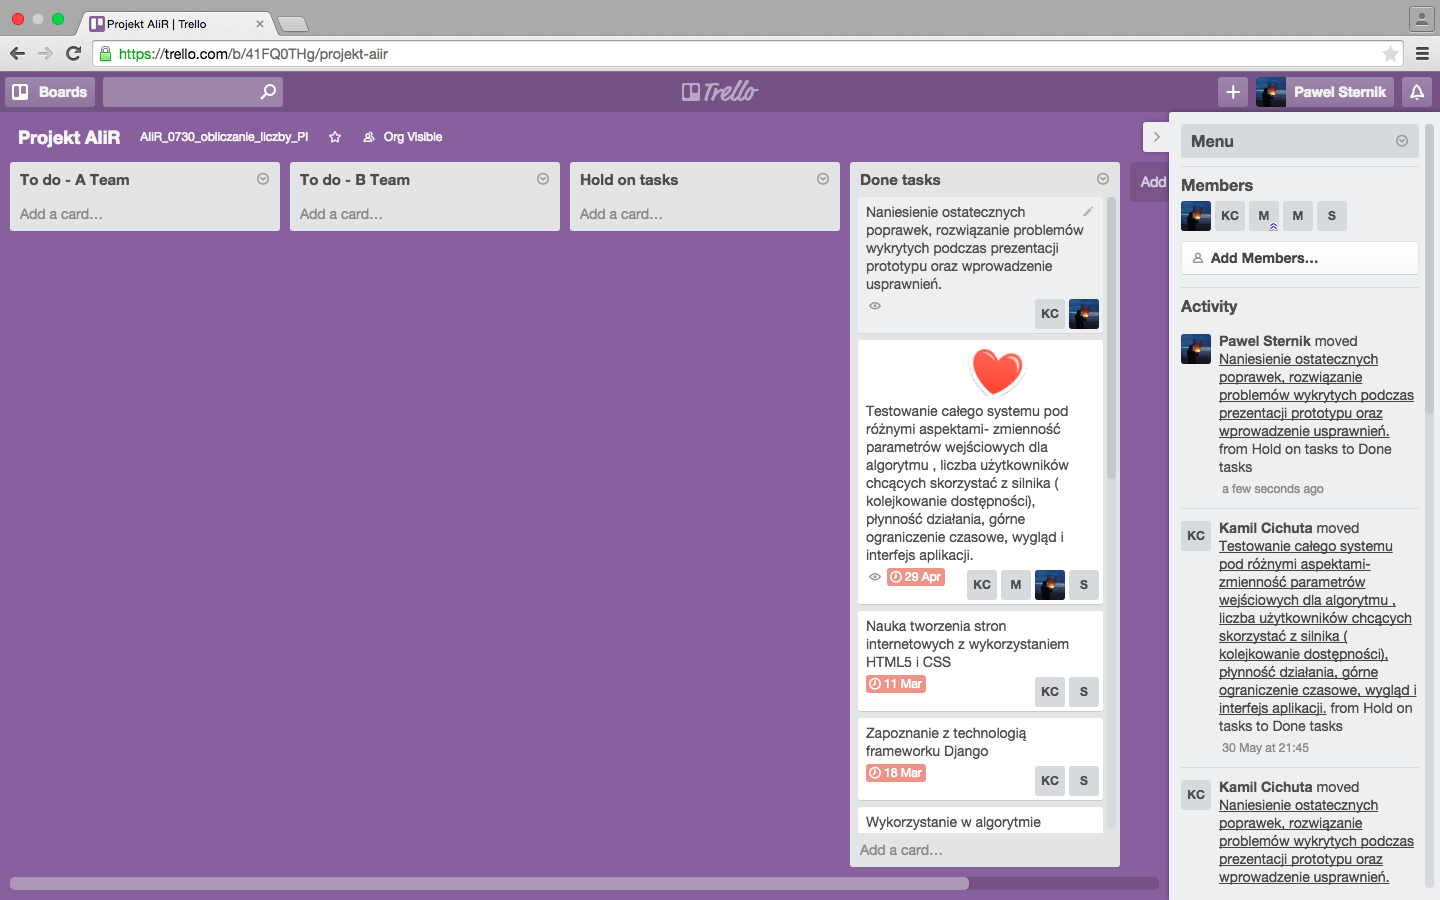
\includegraphics[scale=0.2]{Resources/Trello_Zrzut.png}
\caption{Przykłądowy widok tablicy na portalu Trello.} 
\end{figure} 
\section{Plan realizacji.}
\section{Implementacja silnika obliczeniowego.}
\section{Aplikacja internetowa.}
\section{Testy.}
\section{Podsumowanie i wnioski.}

\end{document}
